\section{Quality of the runs}
\label{app:setup}

\begin{itemize}
\item \textbf{Convergence}: $(\max C_D - \min C_D)/\overline{C_D}$ of \zone{wall\_nose} over the last 500
iterations is \val{conv-lo}--\val{conv-hi}\,\% in all eight runs, below the \SI{0.1}{\percent} of REPORT-4
(Figure~\ref{fig:cdhist}).
\item \textbf{Wall resolution}: over the eight runs, the largest $y^+$ is \val{yplus-nose} on the nose and
\val{yplus-coupler} on the coupler (Figure~\ref{fig:yplus} shows burnout), so the boundary layer is resolved
down to the wall as SST requires.
\item \textbf{Mesh}: the REPORT-4 recipe, 174\,380 (A) and 174\,155 (B) cells, maximum skewness 0.90 and
0.94. No mesh study was made for these two noses; the recipe was checked on study~A only.
\end{itemize}

\begin{figure}[H]
\centering
\begin{subfigure}[t]{0.49\linewidth}
\centering
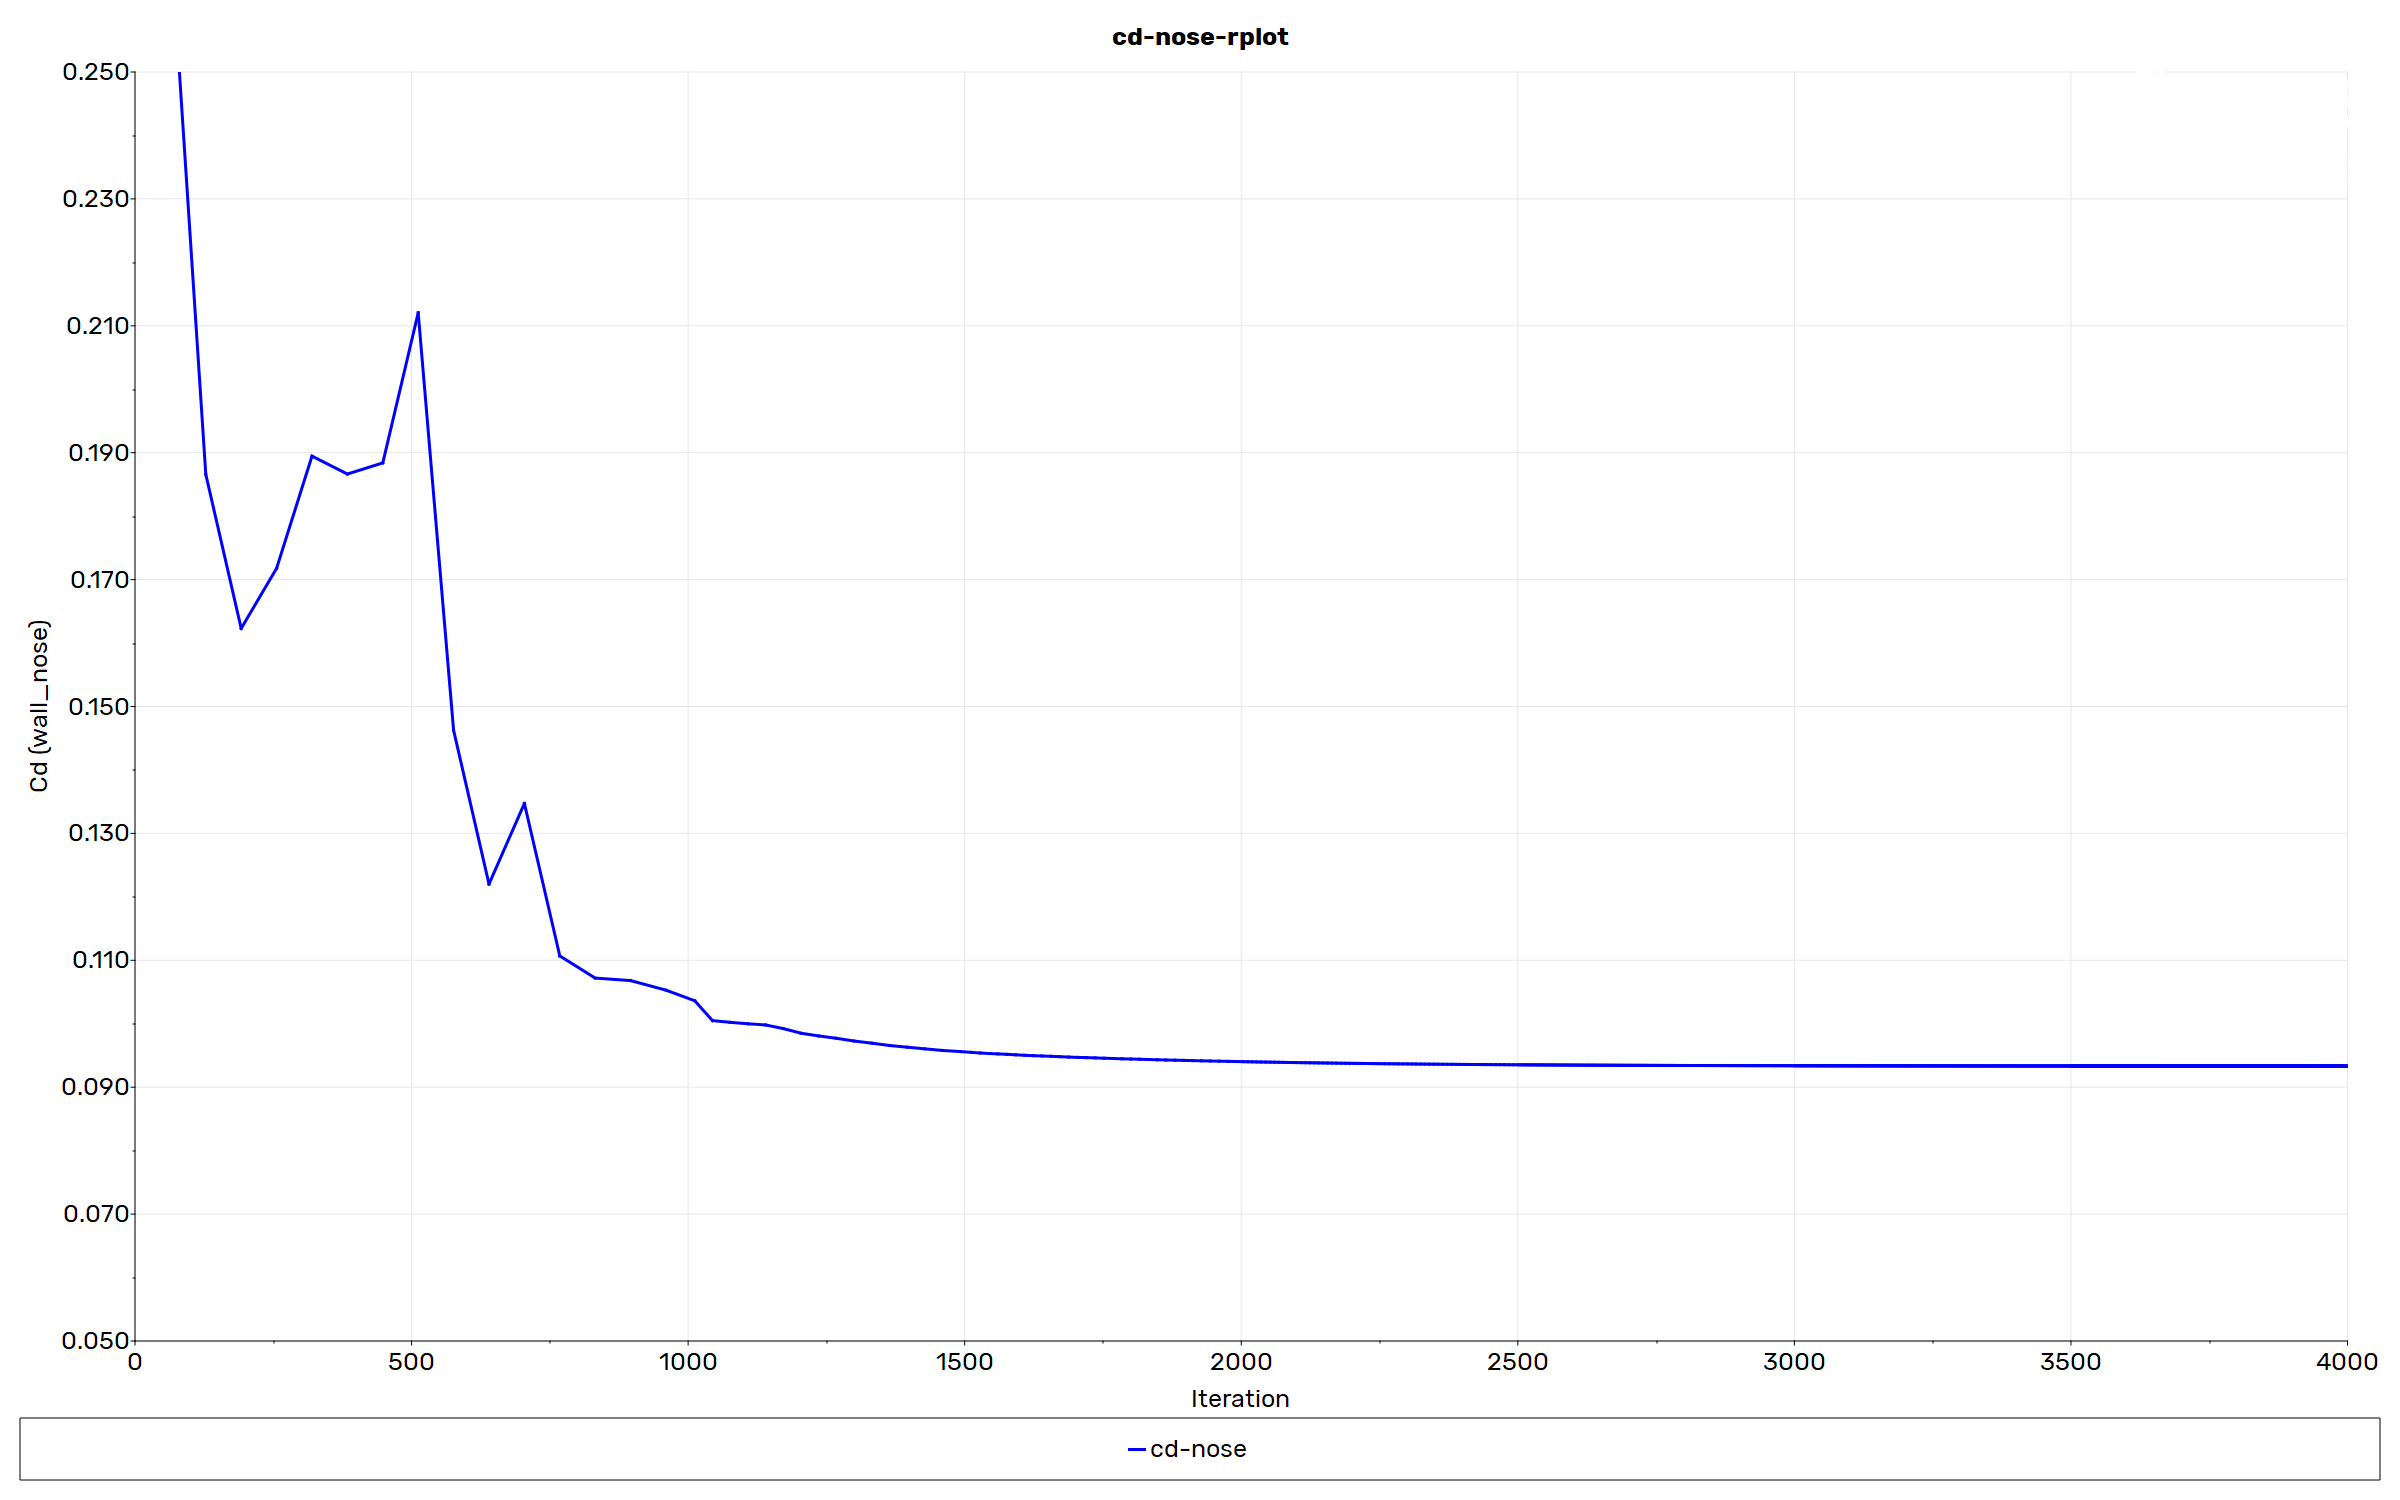
\includegraphics[width=\linewidth]{fluent_cd_A_adiab}
\caption{Design A, burnout.}
\end{subfigure}\hfill
\begin{subfigure}[t]{0.49\linewidth}
\centering
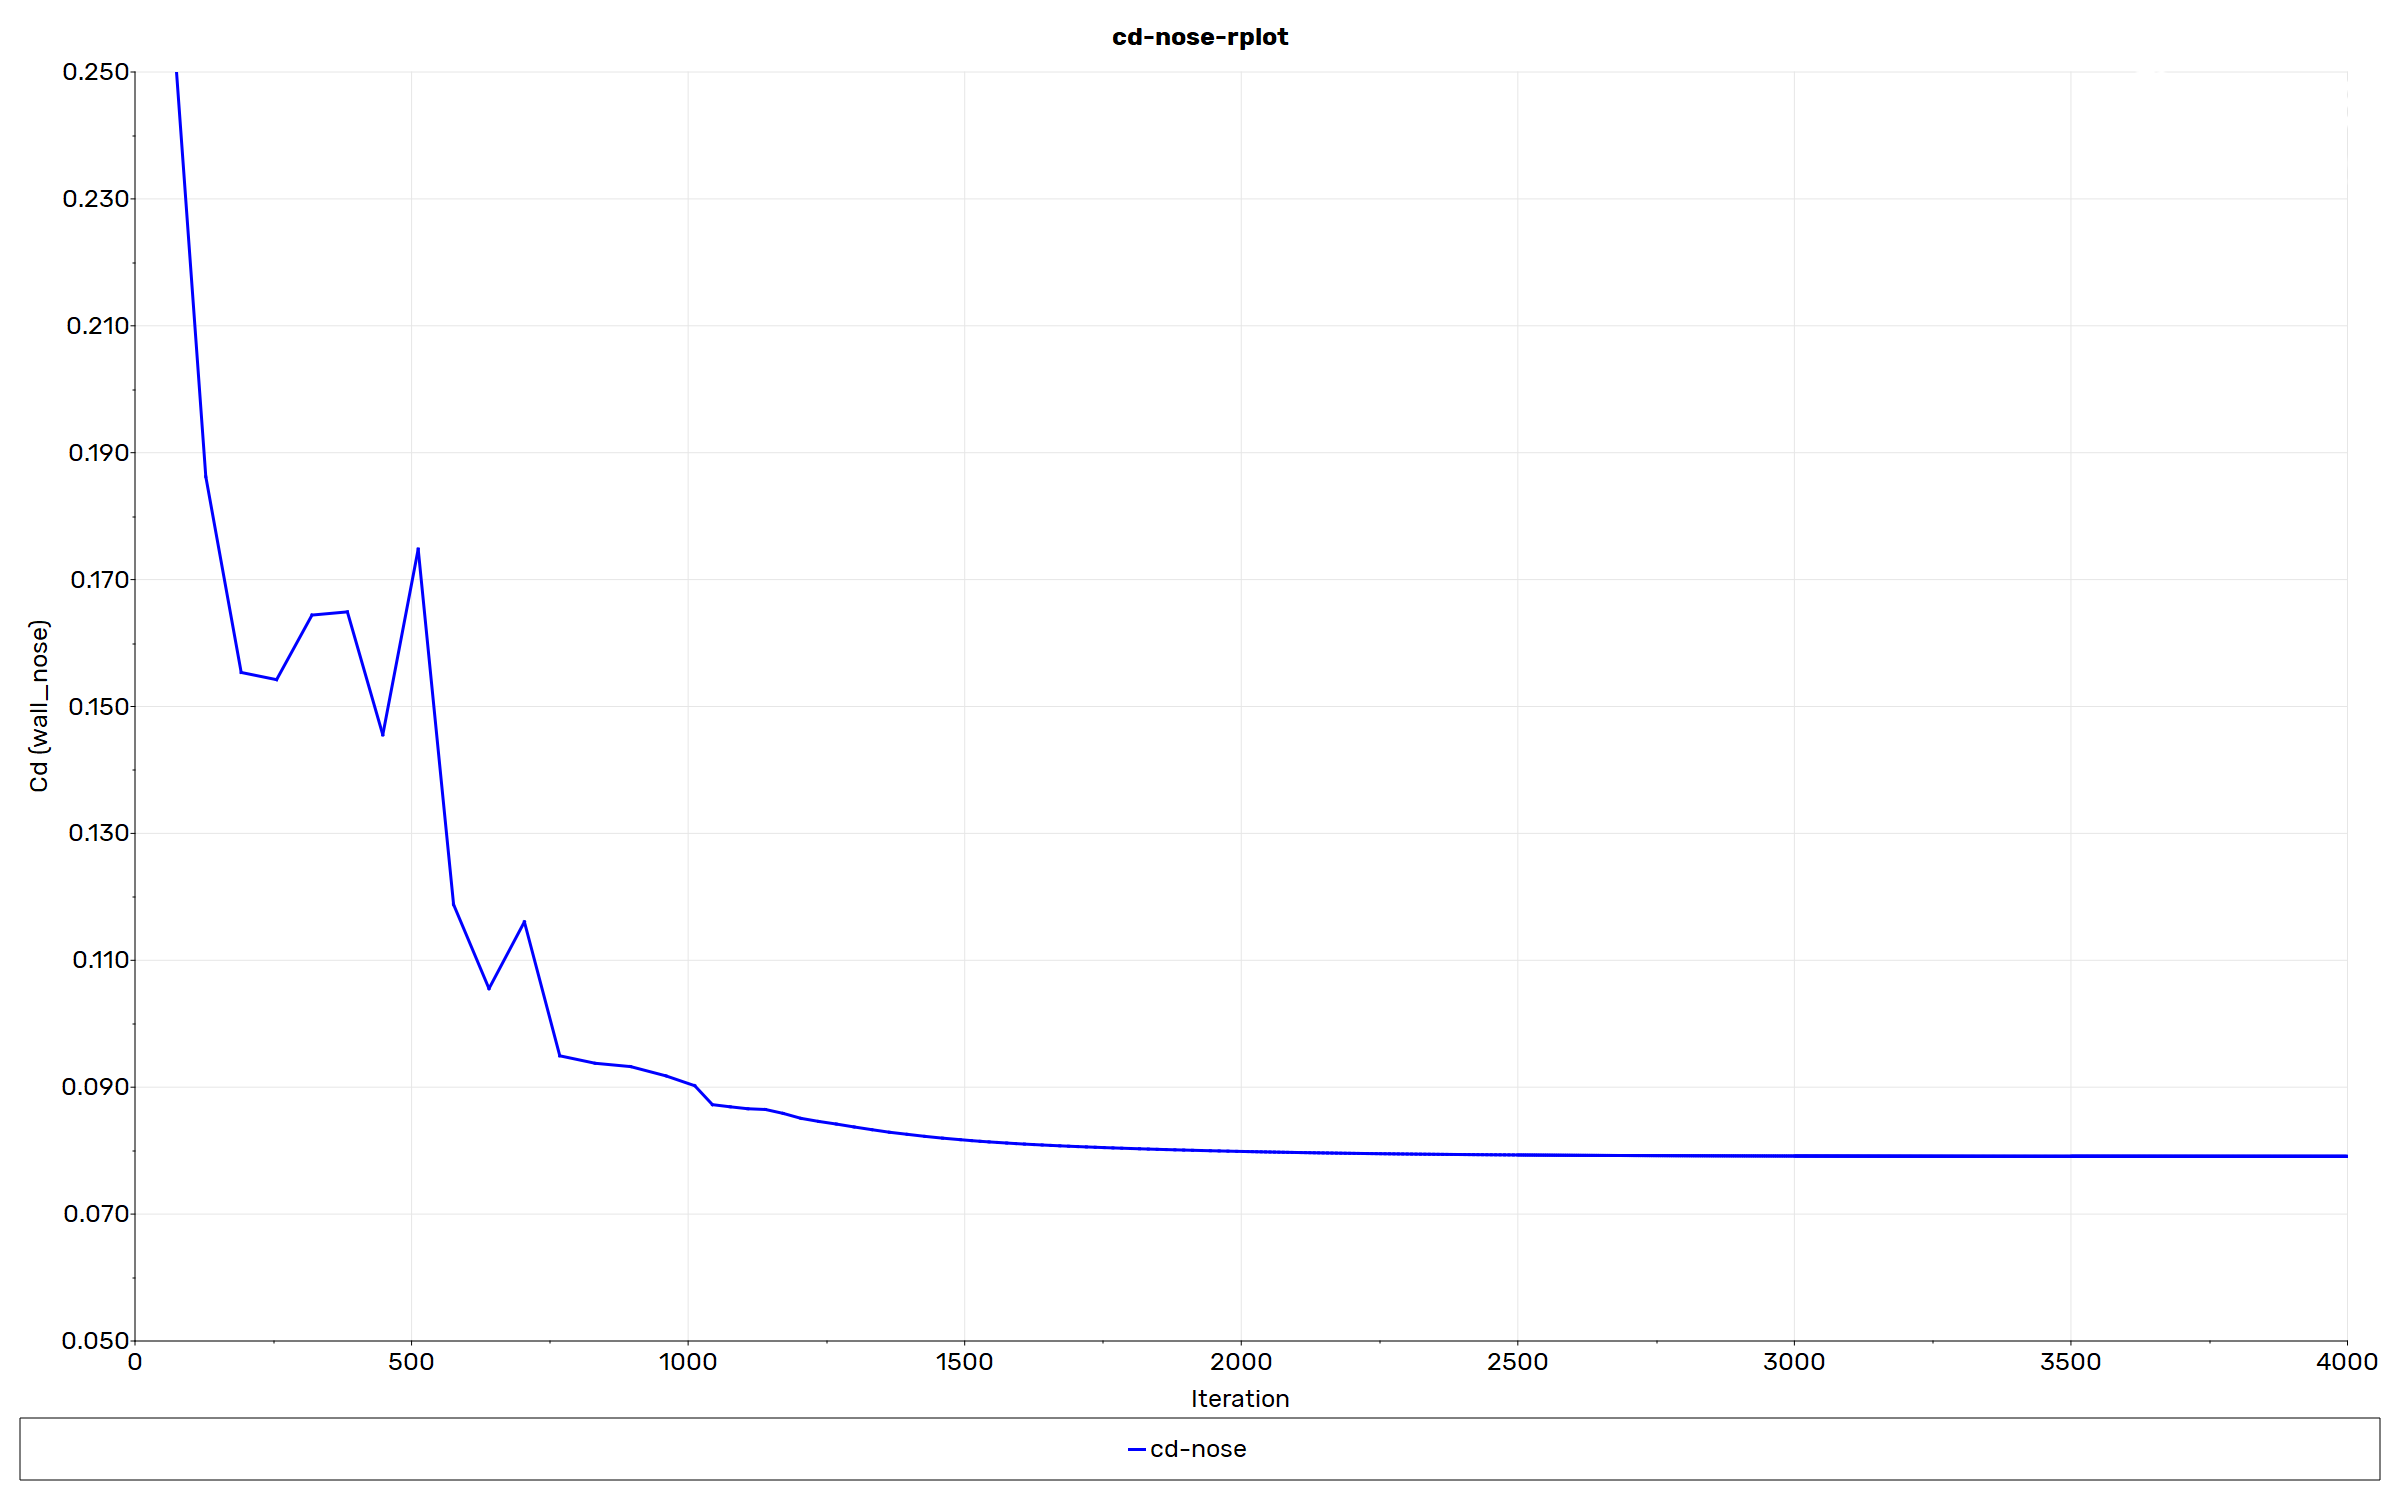
\includegraphics[width=\linewidth]{fluent_cd_B_adiab}
\caption{Design B, burnout.}
\end{subfigure}
\caption{Drag coefficient against iterations (Fluent).}
\label{fig:cdhist}
\end{figure}

\begin{figure}[H]
\centering
\begin{subfigure}[t]{0.49\linewidth}
\centering
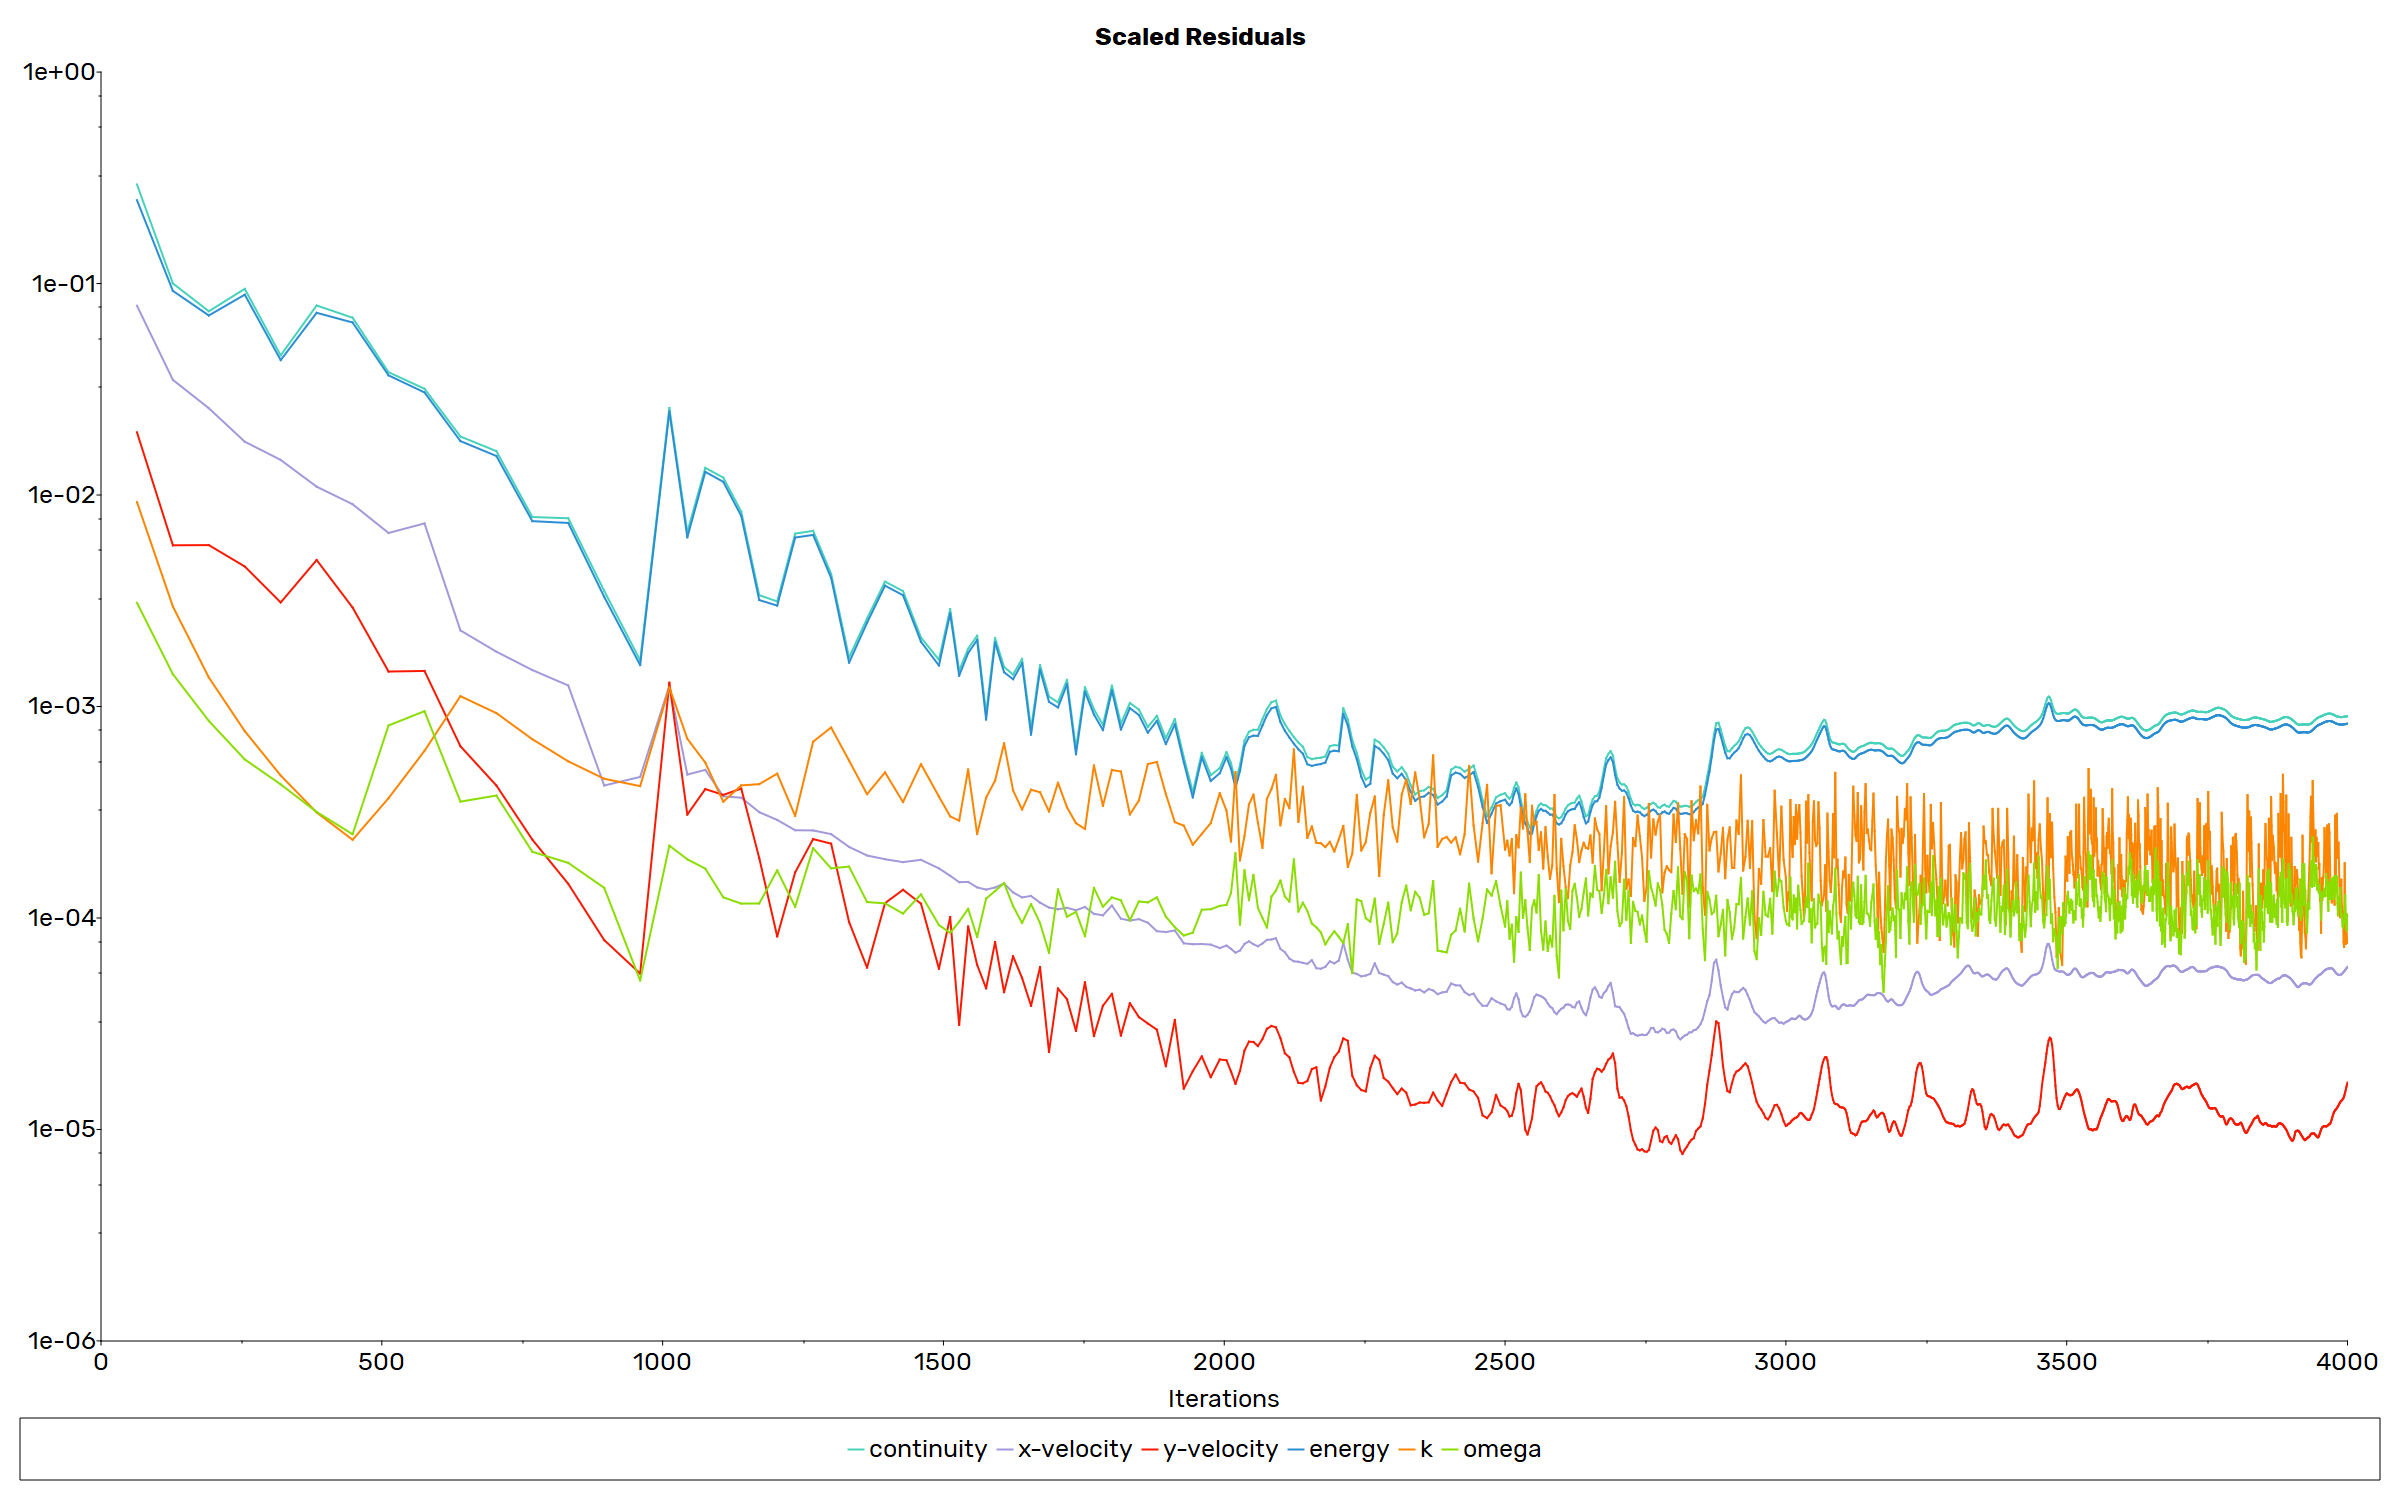
\includegraphics[width=\linewidth]{fluent_residuals_A_adiab}
\caption{Design A, burnout.}
\end{subfigure}\hfill
\begin{subfigure}[t]{0.49\linewidth}
\centering
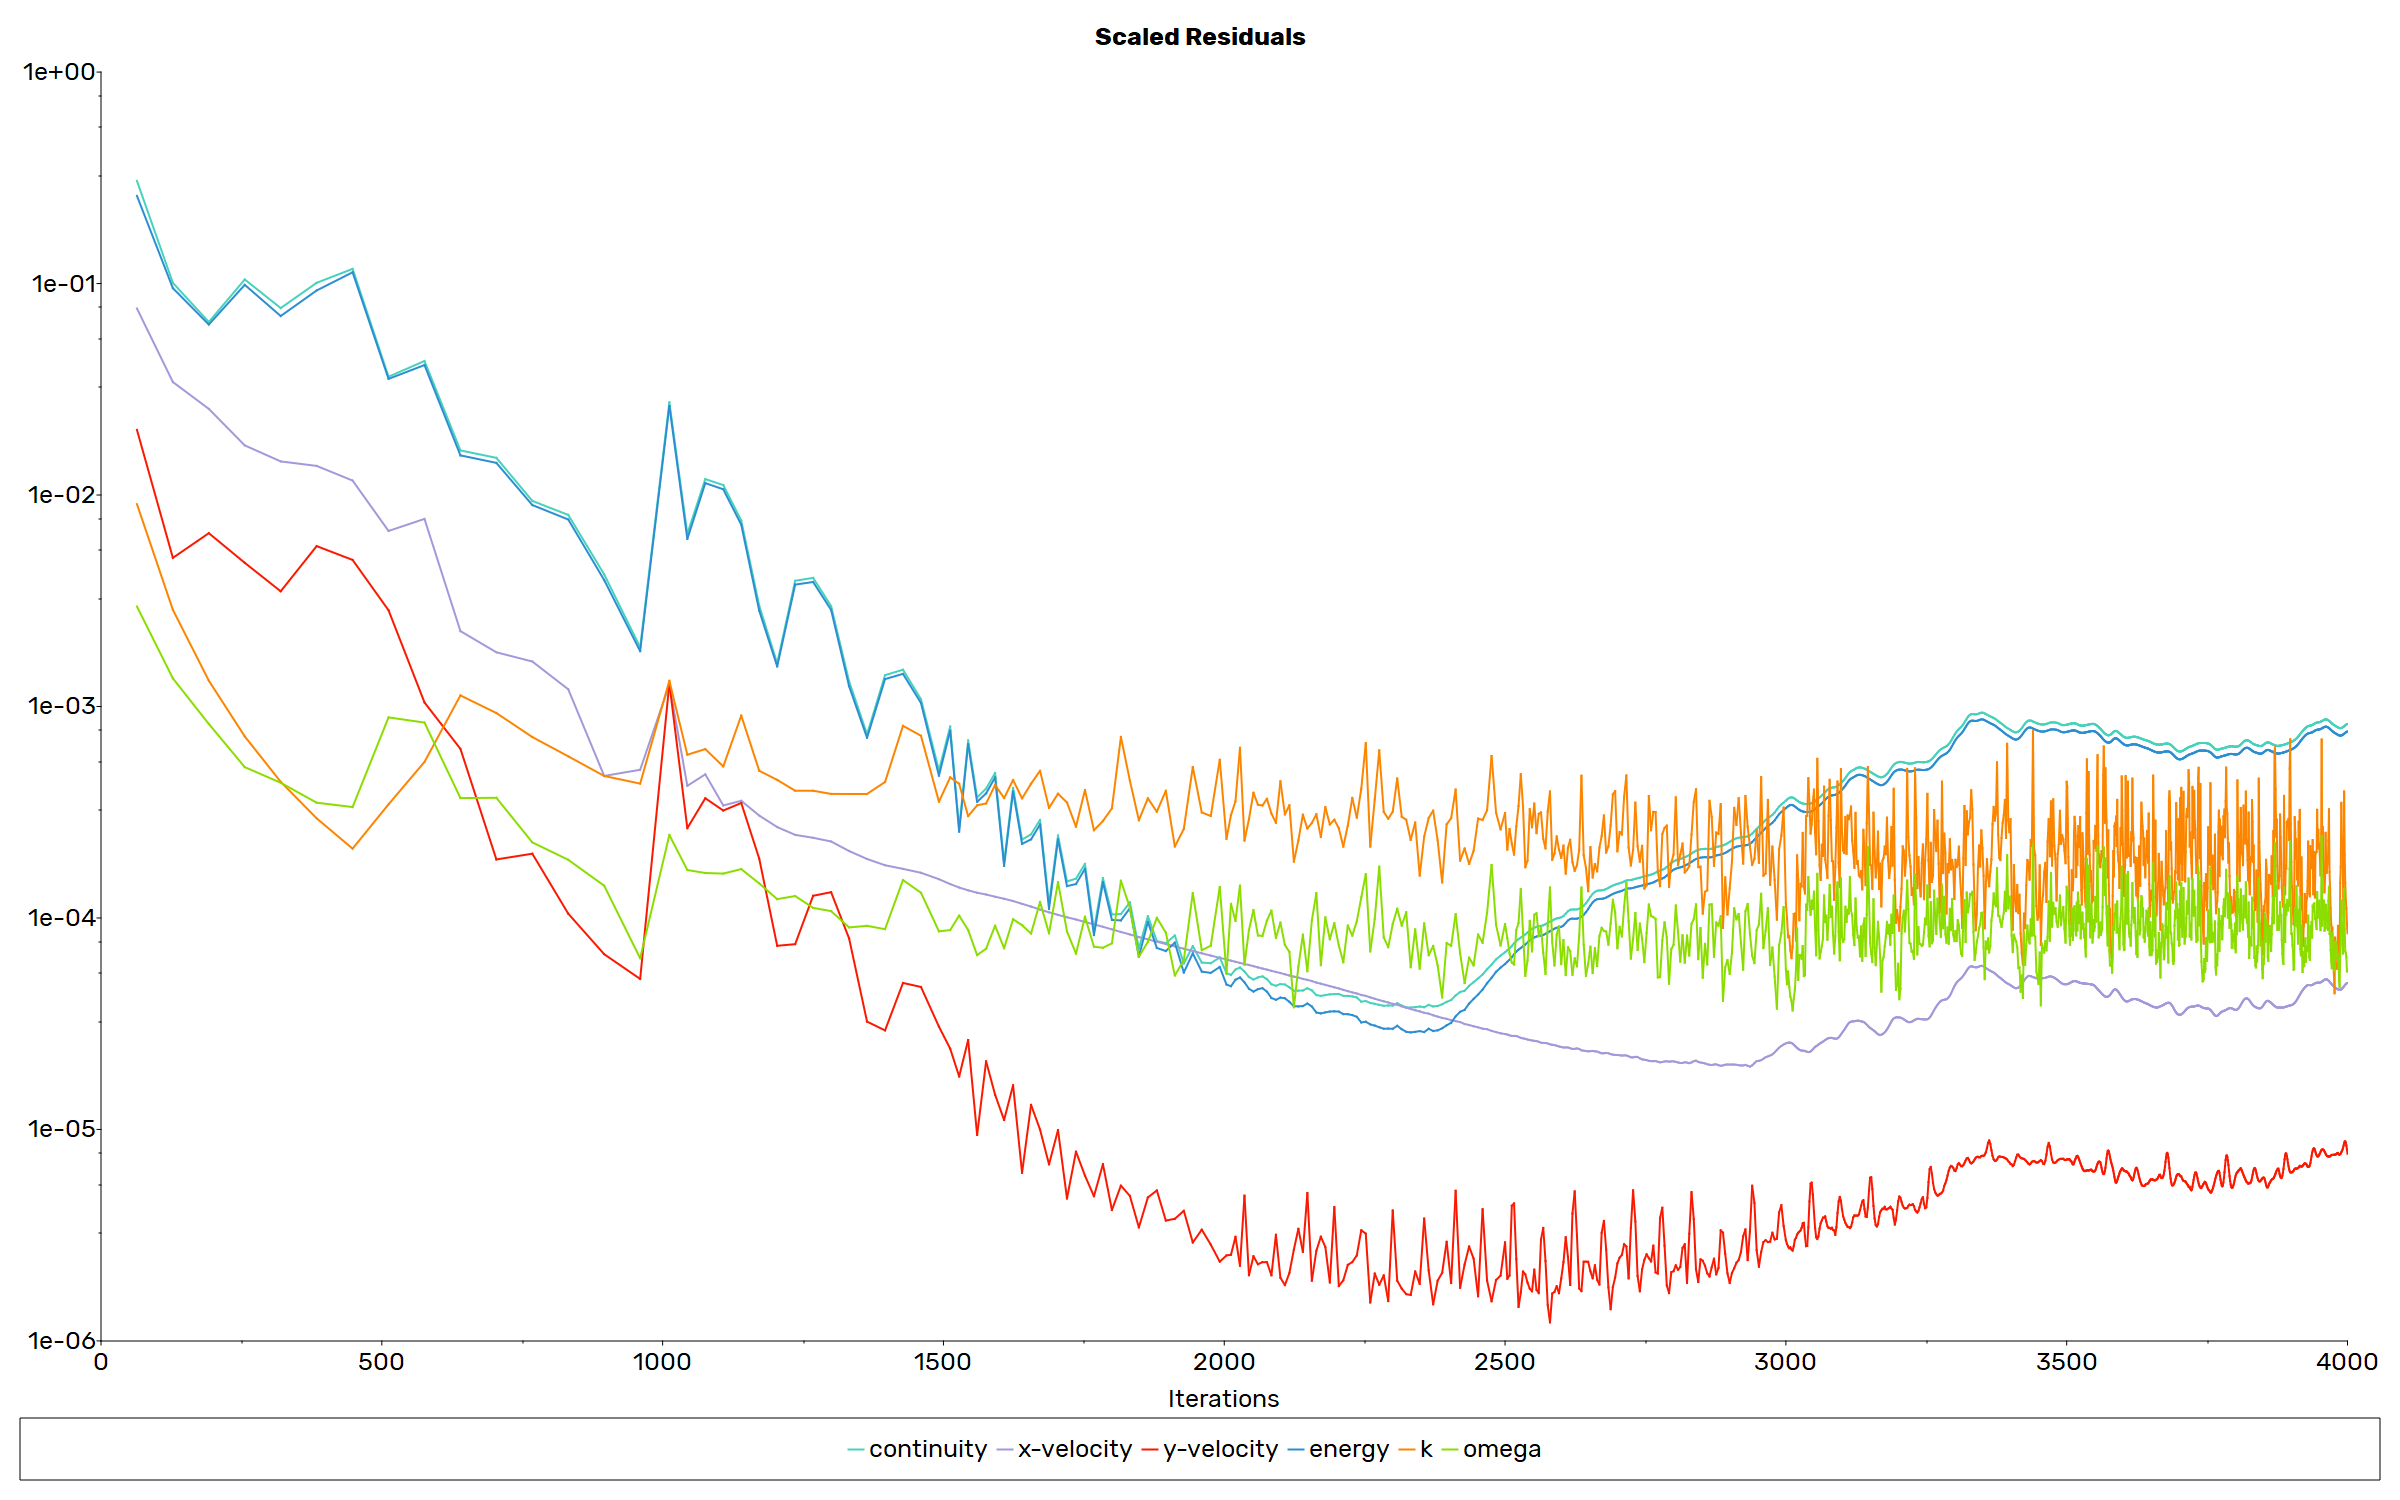
\includegraphics[width=\linewidth]{fluent_residuals_B_adiab}
\caption{Design B, burnout.}
\end{subfigure}
\caption{Residuals against iterations (Fluent).}
\label{fig:residuals}
\end{figure}

\begin{figure}[H]
\centering
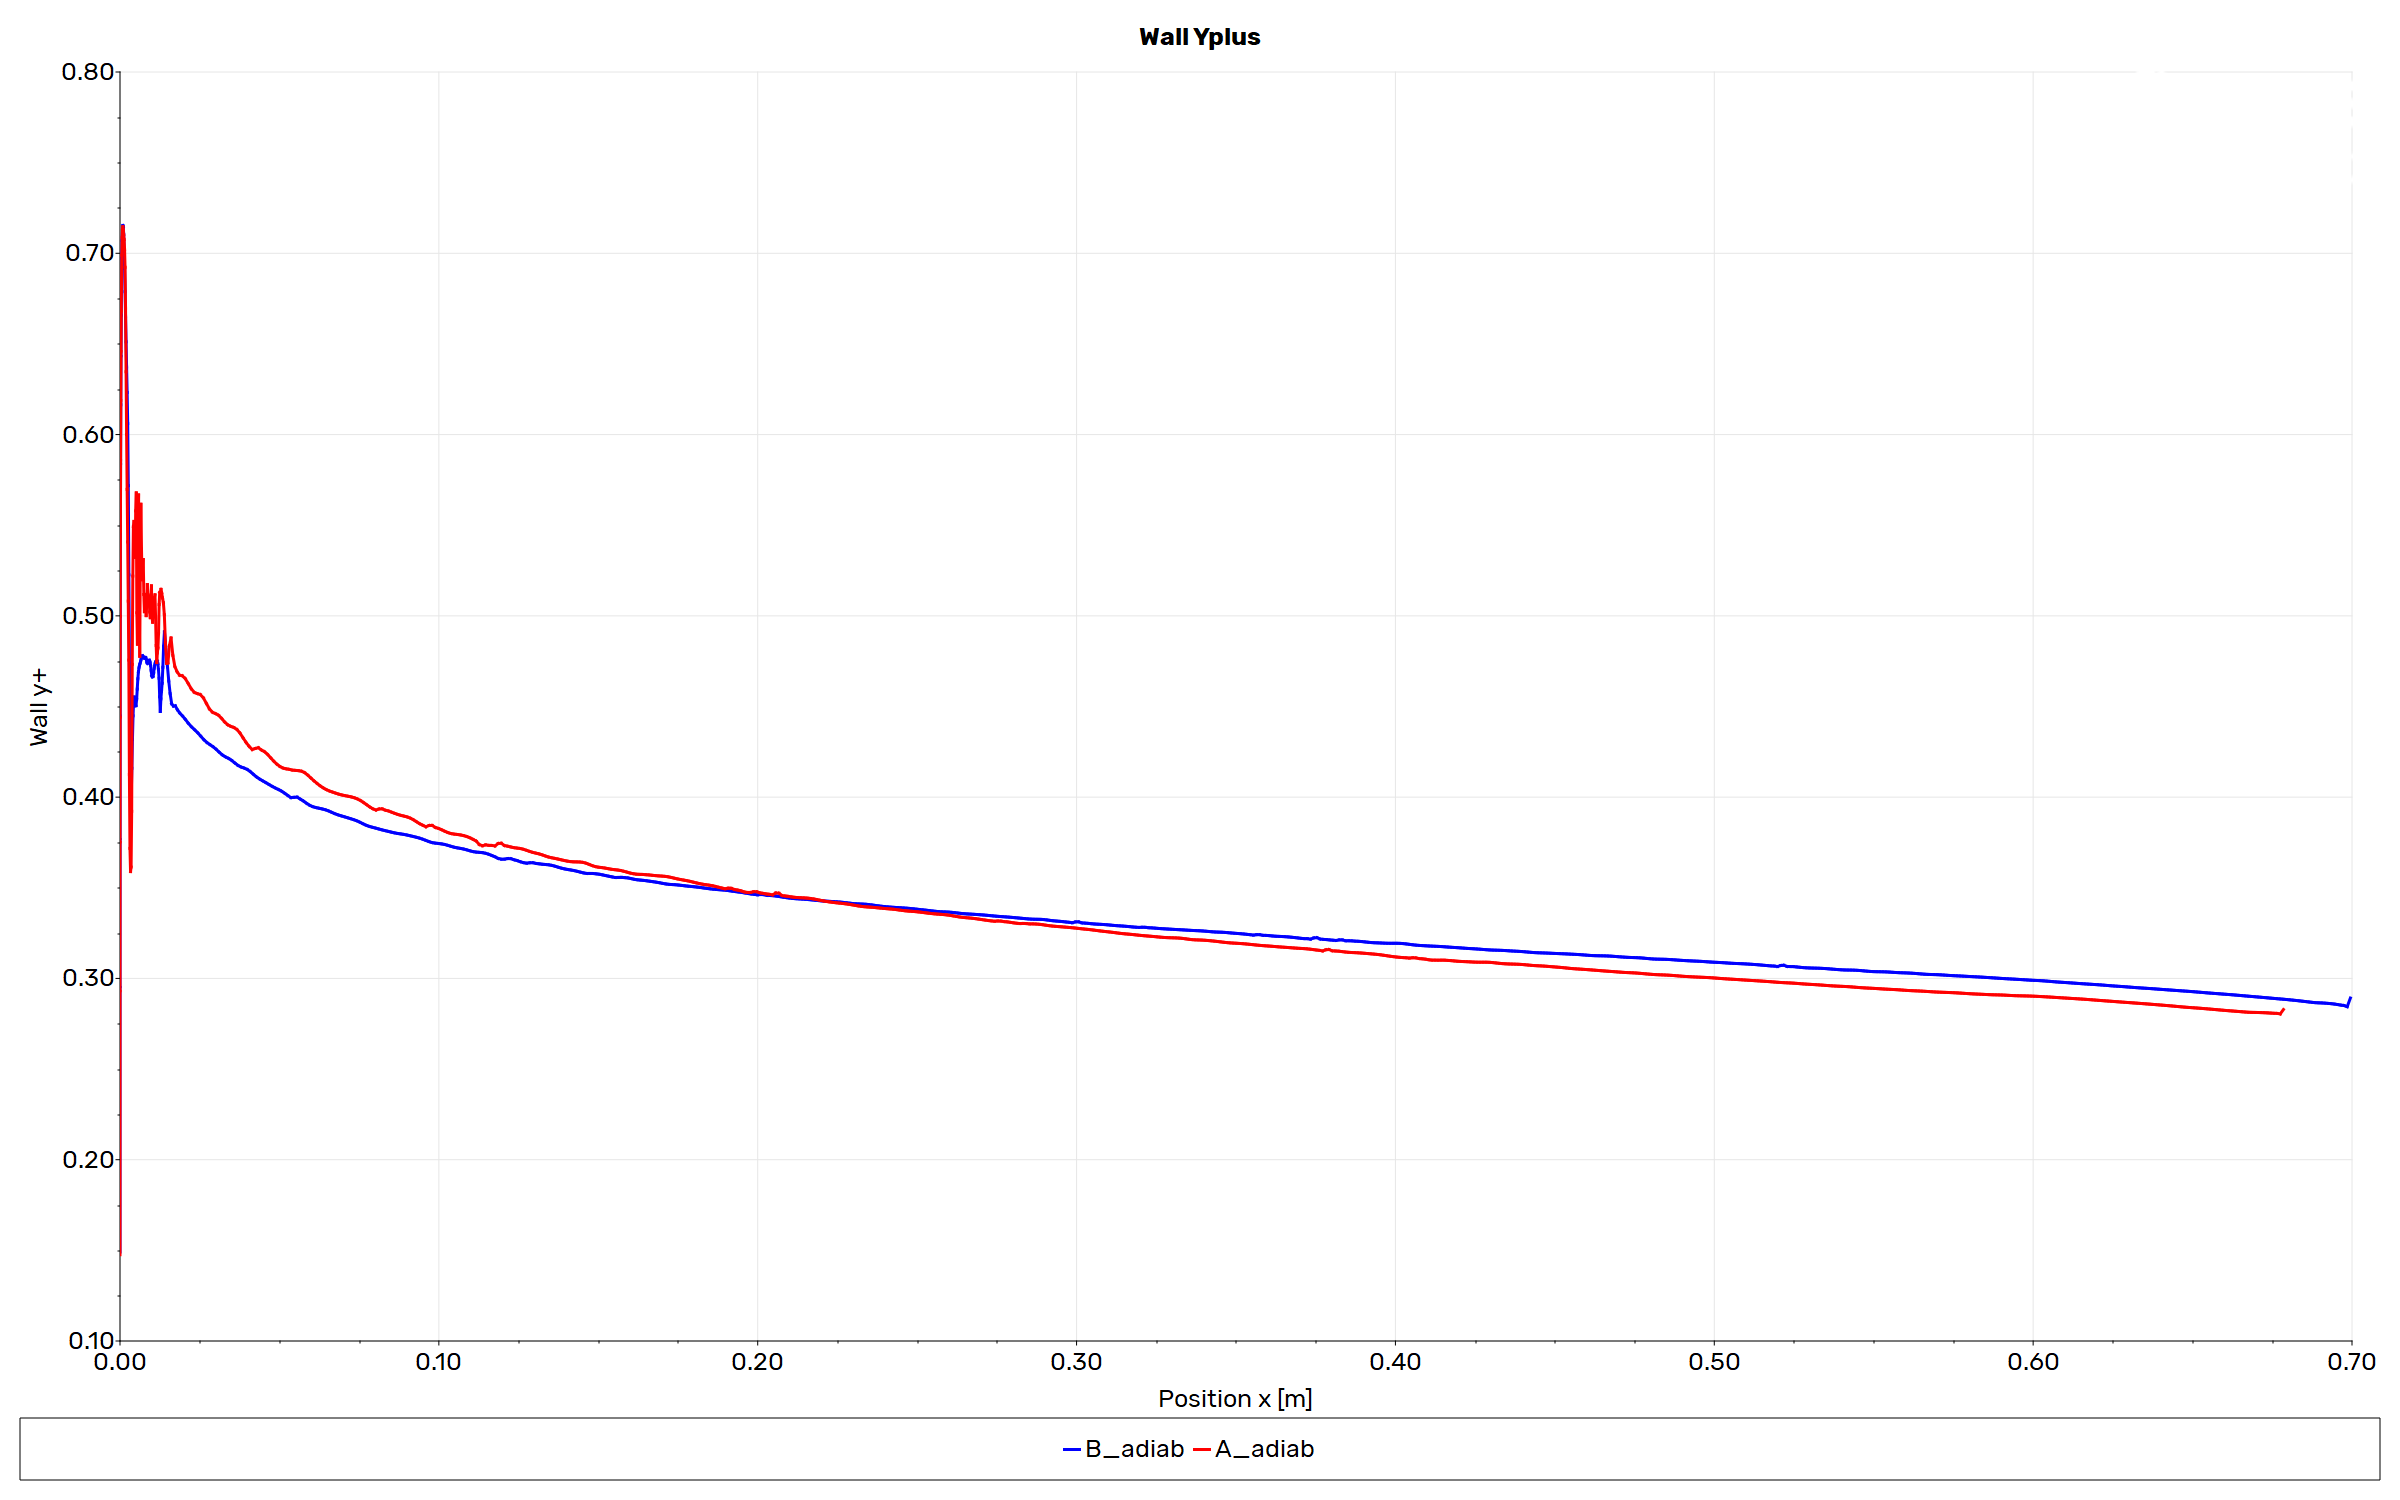
\includegraphics[width=\linewidth]{fluent_yplus_AB_adiab}
\caption{$y^+$ of the first cell along the wall at burnout, design A (red) and B (blue), Fluent.}
\label{fig:yplus}
\end{figure}
